%!TEX root = ../main.tex

\chapter {Evaluation}
\label {cha:evaluation}
This chapter contains interesting IEC functions and procedures, either found in production code or collected and translated from literature.
Each example provides the code, the control flow graph, a description and some metrics, like execution time, number of instruction blocks needed to conclude the result and, most importantly, the reported violations.


\section{Basic Example}
This example in Figure \ref{code:basic example 1 cfg} was found in production code and motivation for this implementation and thesis. There are no loops or procedure calls present, which change the variables provided as parameters (even though there are procedure calls, they cannot change them, since they are only declared as input variables).
Basically, this algorithm contains simple assignments and conditions, which eventually lead to unreachable code when combined, only.
As described at Figure \ref{code:basic example 1}, basic block 11 is not reachable, a consequence of the condition in line 15.
Even though a simple example on how unreachable code may look like in production code, it is easily demonstrated how code becomes unreachable by conditions, when they are combined.
The idea of the implementation originated from this example.

Metrics:
\begin{itemize}
	\item Runtime: 581 ms
	\item Number of analyzed instruction blocks: 17
	\item Violations: block 11
\end{itemize}

% 581ms
% 17 Blöcke analysiert
% Violation für block 11

\begin{figure}
	\begin{GenericCode}
IF s_operationHour <> m_operationHour THEN
	m_operationHour := s_operationHour;
	IF s_operationHour = 0 THEN
		RESET_ALARM(Name := er_service, SubID1 := m_iNumber);
	END_IF;
	RETURN;
END_IF;
// s_operationHour must be equal to m_operationHour
IF s_operationHour = 0 THEN
	// unnecessary - already zero
	m_operationHour := 0;
	RESET_ALARM(Name := er_service, SubID1 := m_iNumber);
ELSE
	// unreachable
	IF s_operationHour <> m_operationHour THEN
		s_operationHour := m_operationHour;
	END_IF;
END_IF;	\end{GenericCode}
	\centering

	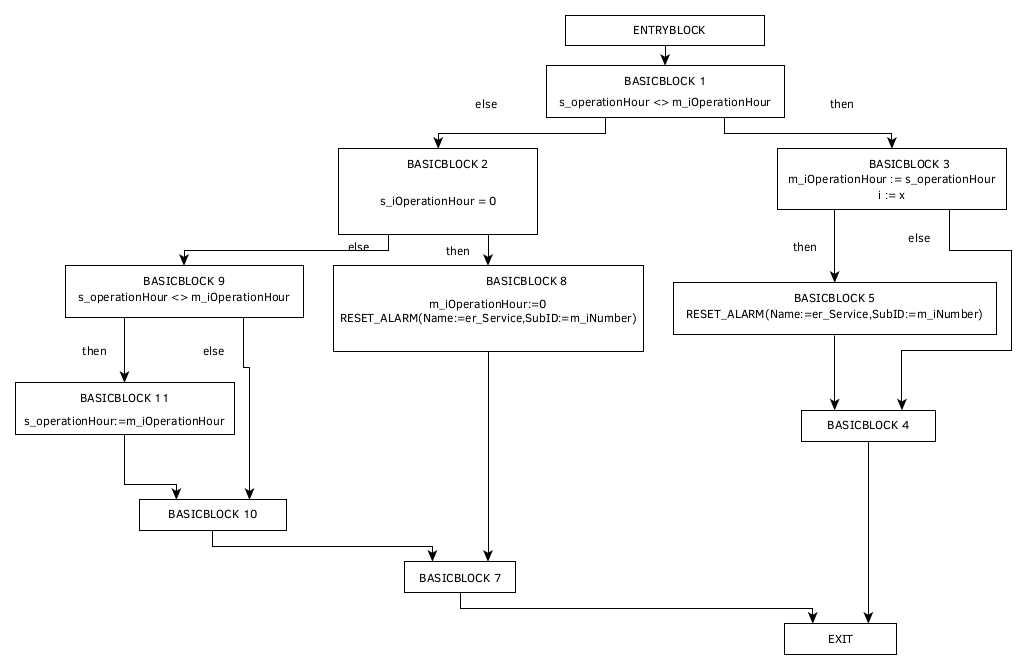
\includegraphics[width=0.9\textwidth]{minimal-example-cfg}
	\caption{A minimal example containing unreachable code due to unsatisfiable conditions. The condition in line 15 is never reachable, since this case was already handled in line 1 and the state of that variable did not change. Therefore basic block 11 is not reachable.}
	\label{code:basic example 1 cfg}
\end{figure}

\begin{figure}
	\centering
	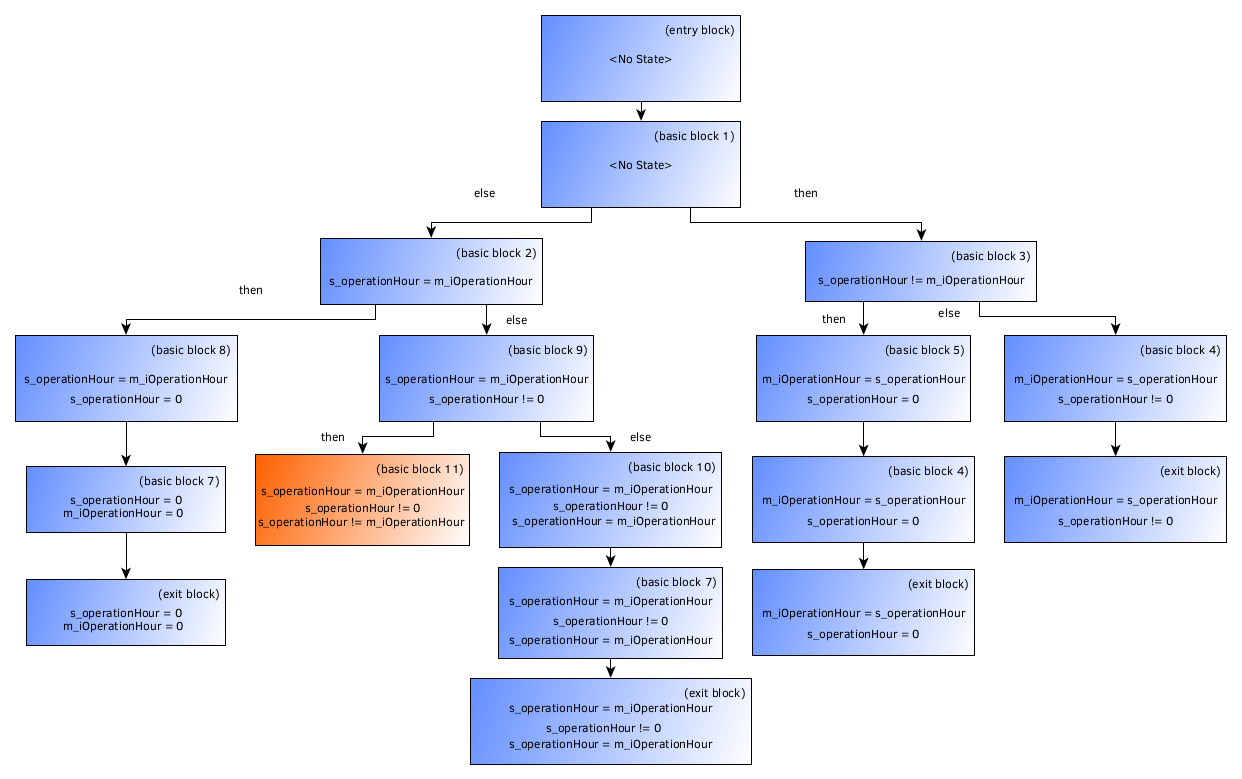
\includegraphics[width=1\textwidth]{minimal-example}
	\caption{Analysis of example \ref{code:basic example 1 cfg}. }
	\label{code:basic example 1}
\end{figure}

\section{Loops}
The main consequence of the implementation is significantly greater execution time, especially, when loops are present.
The following examples contain an almost identical algorithm. The only difference is that the first example in figure \ref{code:loop example 1 cfg} has a set value for x, whereas the example in figure \ref{code:loop example 2 cfg} does not have a limitation. Therefore basic block 6 is not reachable in the first example in figure \ref{code:loop example 1}, but may be reachable for the second example in figure \ref{code:loop example 2}.


Metrics (Example 1):
\begin{itemize}
	\item Runtime: 61 ms
	\item Number of analyzed instruction blocks: 20
	\item Violations: block 6
\end{itemize}



Metrics (Example 2):
\begin{itemize}
	\item Runtime: <1 ms
	\item Number of analyzed instruction blocks: 68
	\item Violations: none
\end{itemize}


\begin{figure}
	\begin{GenericCode}
i := 1;
x := 5;
		
WHILE i < x DO
	i := i + 1;
END_WHILE;
		
IF i = 3 THEN
	x := 4;
END_IF;	\end{GenericCode}
	\centering
	% 61ms
	% 20
	% Violation für block 6
	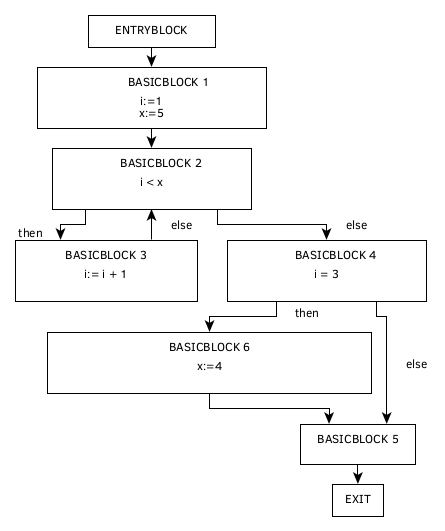
\includegraphics[width=0.6\textwidth]{basic-while-cfg}
	\caption{The variable i will change inside the loop. As long as x is not equal to 3, the basic block 6 is unreachable. }
	\label{code:loop example 1 cfg}
\end{figure}
\begin{figure}
	\centering
	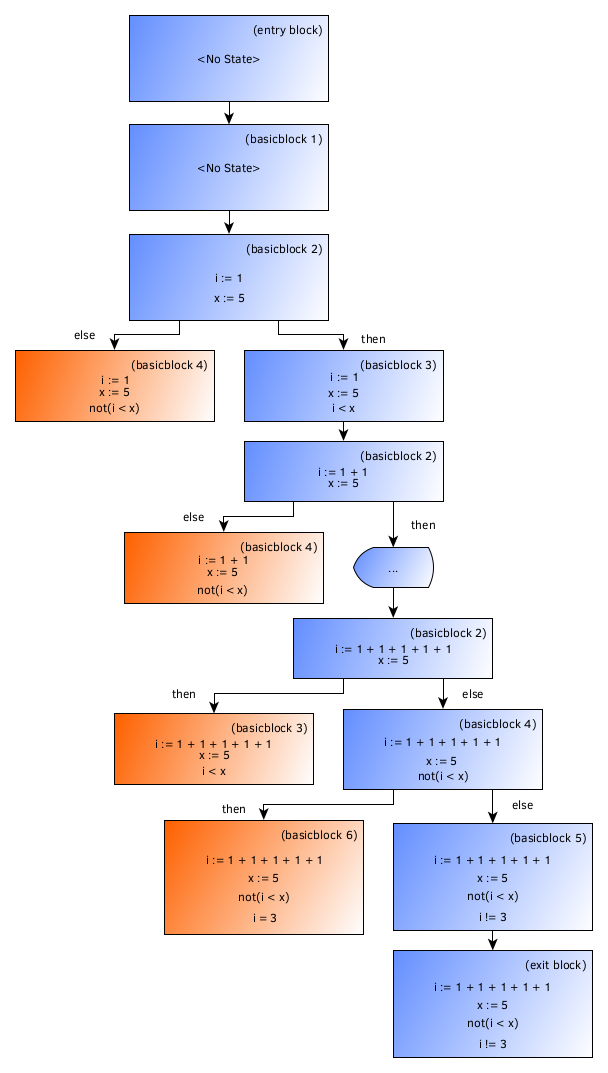
\includegraphics[width=0.6\textwidth]{basic-while}
	\caption{Analysis of example \ref{code:loop example 1 cfg}. }
	\label{code:loop example 1}
\end{figure}
\begin{figure}
	\begin{GenericCode}
i := 1;
		
WHILE i < x DO
	i := i + 1;
END_WHILE;
		
IF i = 3 THEN
	x := 4;
END_IF;		\end{GenericCode}
	\centering
	% <1ms
	% 68
	% No violations
	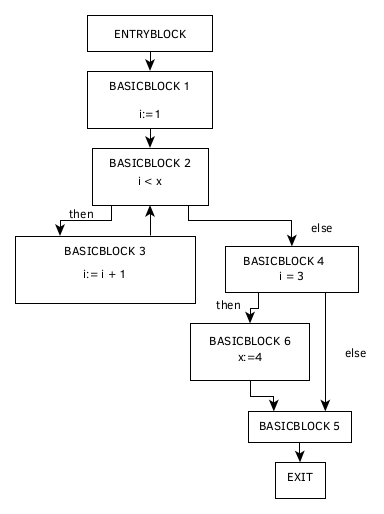
\includegraphics[width=0.6\textwidth]{basic-while-input-cfg}
	\caption{Same as \ref{code:loop example 1}, but x is an input variable. Therefore it may be 3, so it could be reachable.}
	\label{code:loop example 2 cfg}
\end{figure}
\begin{figure}
	\centering
	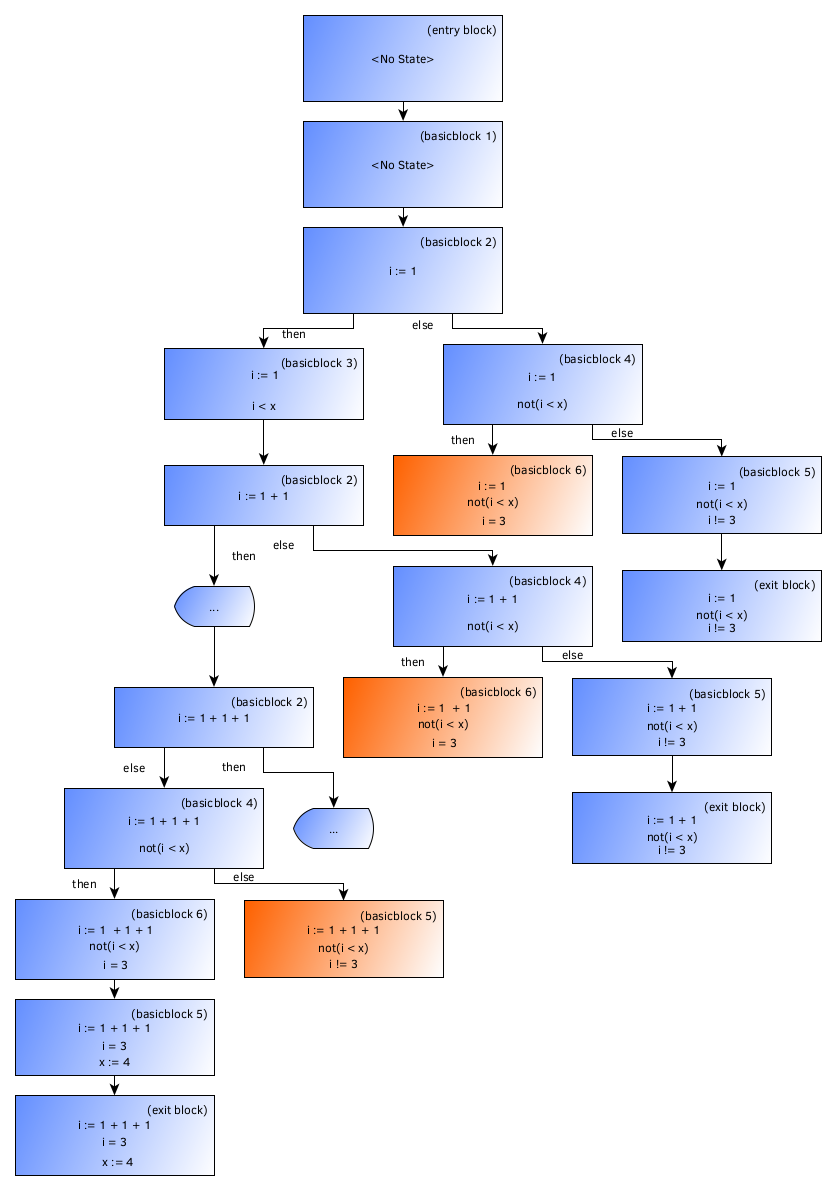
\includegraphics[width=0.8\textwidth]{basic-while-input}
	\caption{Analysis of example \ref{code:loop example 2 cfg}.}
	\label{code:loop example 2}
\end{figure}
\section{Function- and Procedure-Calls}
This example in Listing \ref{code:func test 1} demonstrates the handling of function- and procedure calls. It contains 2 different procedures: FooOutput and algo1 (which is part of an instantiated algorithm block). 
As described in Section, \ref{sub:handling procedure and function calls} only the declaration of parameters matters. Even if the function does not actually change the variable, it will be handled as such. 
Due to these circumstances, basic blocks 5 and 9 are not reachable.


Metrics:
\begin{itemize}
	\item Runtime: 169 ms
	\item Number of analyzed instruction blocks: 31
	\item Violations: block 5
\end{itemize}


\begin{program}
	\begin{GenericCode}
tmp1 := 1;
tmp2 := 2;
tmp3 := 3;

FooOutput(tmp1, tmp2, tmp3);

IF tmp2 <> 2 AND tmp3 <> 3 THEN
	tmp2 := 2; // Reachable - could change
END_IF;

IF tmp1 <> 1 THEN
	tmp2 := 3; // Unreachable
END_IF;

ABFunc.algo1(tmp2, tmp1, tmp3);

IF tmp1 <> 1 AND tmp3 <> 1 THEN
	tmp2 := 3; // Reachable
END_IF;

ABFunc.algo1(out1 => tmp1, in1 := tmp2, in_out1 := tmp3);

IF tmp2 = 3 THEN
	tmp2 := 3; // Reachable
END_IF;	\end{GenericCode}
	\centering
	% 169ms
	% 31 
	% Violations 5
	\caption{Demonstrates intraprocedural analysis. The procedure  FooOutput declares the first parameter as an IN parameter and therefore has no effect on the variable, while the other two parameters are declared as OUT parameters and might change. Note that the analysis does not check if the out parameter will be mutated, so it will be counted as if it would have. ABFunc is an instantiated algorithm block, which is similar to a class, and declares the parameters of the procedure \emph{algo1} in the same order. Note that the second occurrence of this method call contains named parameters. \emph{out1} and \emph{in\_out3} may be mutated.}
	\label{code:func test 1}
\end{program}
\begin{figure}
	\centering
	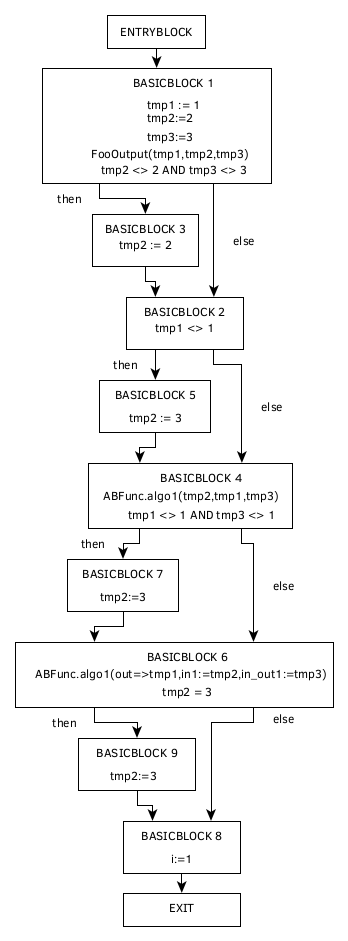
\includegraphics[width=0.5\textwidth]{easy-func-test-cfg}
	\caption{Control flow graph of example \ref{code:func test 1}}
	\label{fig:func test 1 cfg}
\end{figure}
\begin{figure}
	\centering
	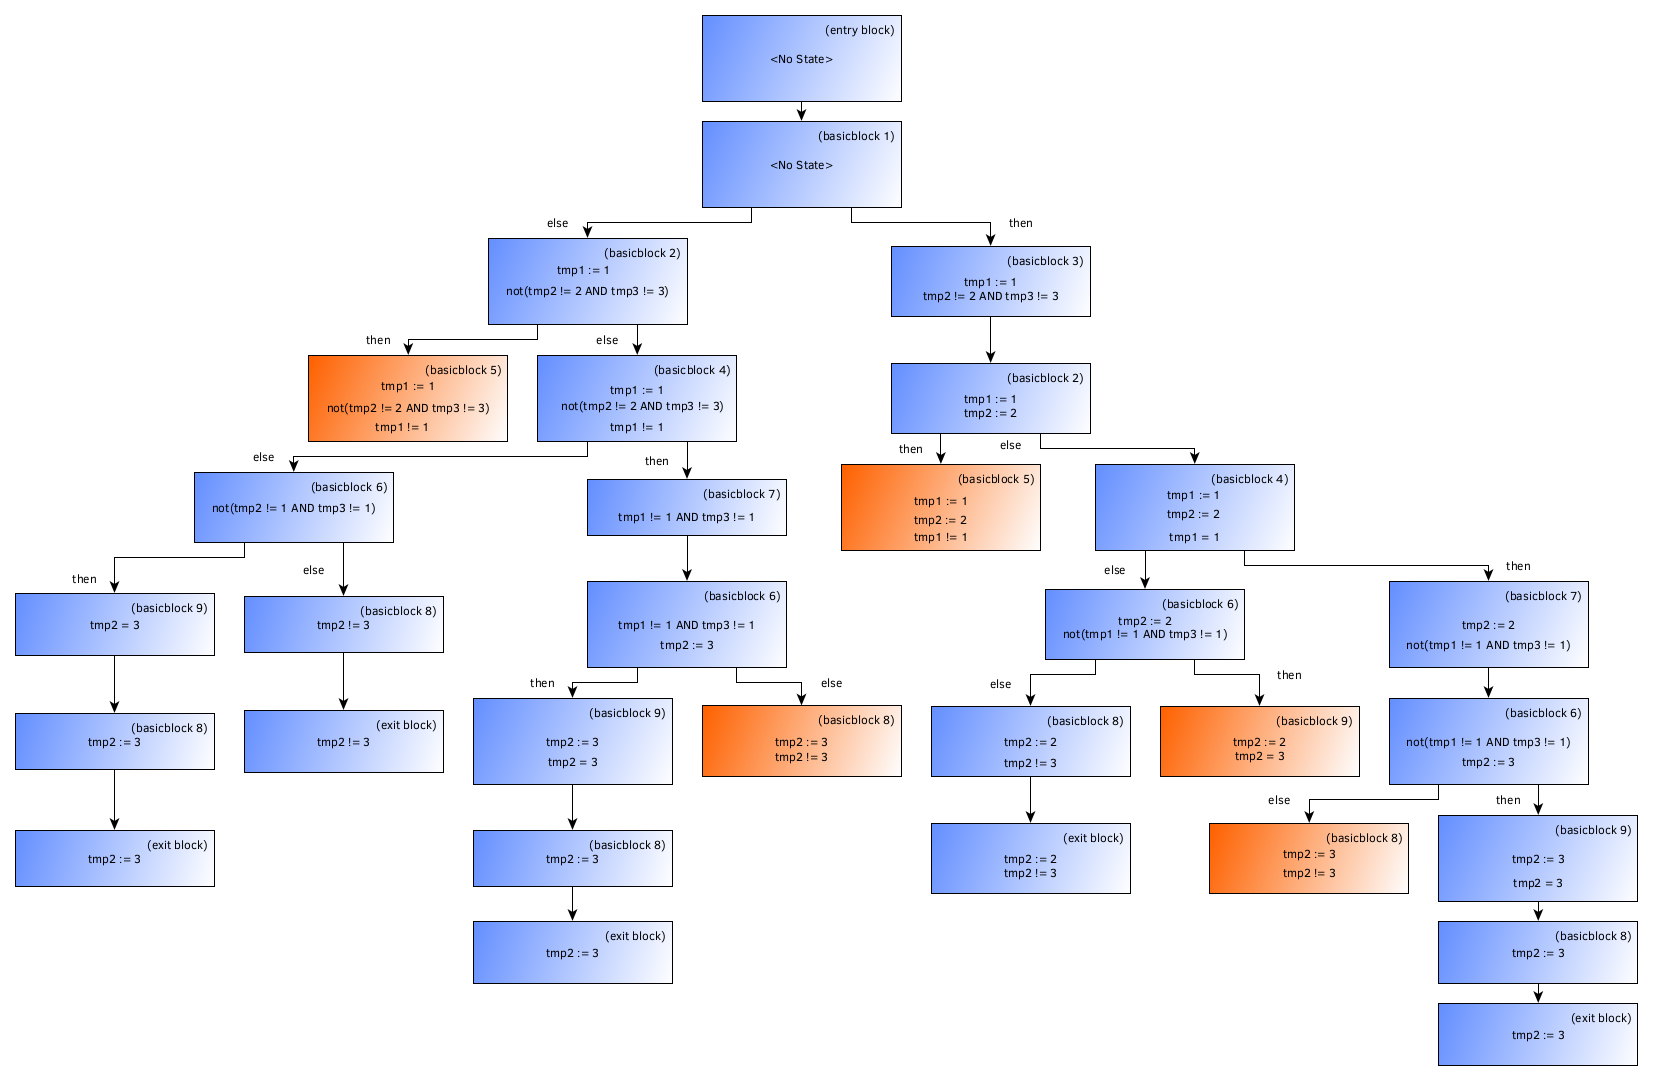
\includegraphics[width=1\textwidth]{easy-func-test}
	\caption{Analysis of example \ref{fig:func test 1 cfg}.}
	\label{fig:func test 1}
\end{figure}

\section{Hard Example}
This example in Figure \ref{code:hard example 1} and Figure \ref{code:hard example 1 cfg} was found in the literature \cite{Click_1995} and it was stated that the usual method for finding unreachable code is not able to detect this instance. 
Since the implementation is different at its core, it was only natural to test and compare the results.
Since no other functions were injected for this analysis, in contrast to the method described in chapter \ref{cha:state of the art}, this instance will be found and reported.
Note that the loop contains a variable which does not change, which will never stop. Therefore the analysis would stop early and no violation would be reported without the correct configuration. 
If the condition would have been different, it is easier to detect, but since this example has been used by different sources it was not altered.


Metrics:
\begin{itemize}
	\item Runtime: 20 ms
	\item Number of analyzed instruction blocks: 47
	\item Violations: block 4
\end{itemize}

\begin{figure}
	\begin{GenericCode}
x := 1;
	
REPEAT
	b := x <> 1;
	IF b = TRUE THEN
		x := 2;
	END_IF;    
UNTIL pred
END_REPEAT;	\end{GenericCode}
	% 20ms
	% 47
	% Violation Block 4
	\centering
	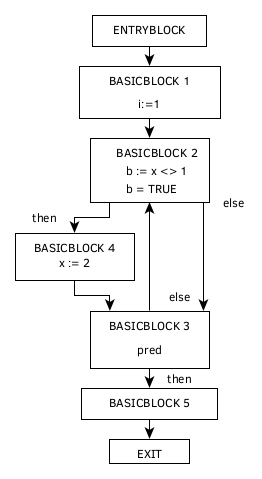
\includegraphics[width=0.4\textwidth]{hard-example-cfg}
	\caption{As described in \ref{code:ssa-defect} this procedure cannot be analyzed correctly and will not report that basic block 4 is unreachable. }
	\label{code:hard example 1}
\end{figure}
\begin{figure}
	\centering
	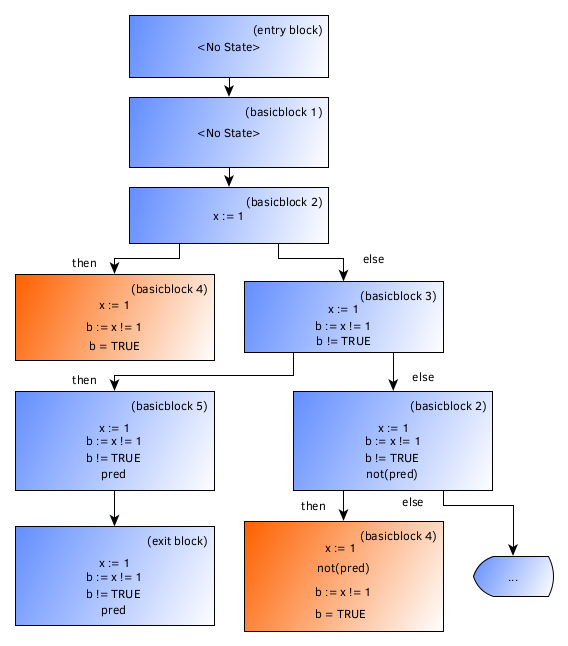
\includegraphics[width=0.7\textwidth]{hard-example}
	\caption{Analysis of example \ref{code:hard example 1 cfg}.}
	\label{code:hard example 1 cfg}
\end{figure}


